\subsubsection{\stid{3.01} hypre} 


\paragraph{Overview} 
The {\sl hypre} software library \cite{hypre:homepage,hypre_design_impl_2006} provides high performance preconditioners and solvers for the solution of large sparse linear systems on massively parallel computers, with particular focus on algebraic multigrid solvers. One of {\sl hypre}’s unique features is the provision of a (semi)-structured interface, in addition to a traditional linear-algebra based interface. The semi-structured interface is appropriate for applications whose grids are mostly structured, but with some unstructured features. Examples include block-structured grids, composite grids in structured adaptive mesh refinement (AMR) applications, and overset grids. These interfaces give application users a more natural means for describing their linear systems, and provide access to methods such as structured multigrid solvers, which can take advantage of the additional information beyond just the matrix. Since current architecture trends are favoring regular compute patterns to achieve high performance, the ability to express structure has become much more important. The {\sl hypre} library provides both unstructured and structured multigrid solvers, which have shown excellent scalability on a variety of high performance computers, e.g Blue Gene systems (unstructured solver BoomerAMG has scaled up to 1.25 million MPI cores with a total of 4.5 million hardware threads). It is used by many ECP application teams, including ExaAM, Subsurface, ExaWind, CEED, and more. It requires a C compiler and an MPI implementation, but it also runs in an OpenMP environment. It has some GPU capabilities.

\paragraph{Key  Challenges}

While {\sl hypre}'s solvers contain much parallelism, their main focus is the solution of sparse linear systems, leading to  very large demands on memory bandwidth. In addition, the use of multiple levels, while greatly aiding convergence of the solvers, leads to decreasing systems sizes, number of operations and parallel efficiencies on coarser levels. Particularly the unstructured algebraic multigrid solver BoomerAMG\cite{HeYa2002}, which is {\sl hypre}'s most often used preconditioner, suffers from increasing communication complexities on coarser levels. Coarse grid operators are generated by multiplying three matrices leading to increasing numbers of nonzeroes per row in the resulting matrices and with it increasing numbers of neighbor processes. While BoomerAMG's solve phase mainly consists of matrix vector products and smoothing operations, which are fairly straight forward to parallelize, even on a GPU, its setup phase is highly complex, including many branches, a lot of integer operations as well as some sequential passages. Current  interpolation strategies that lead to best convergence and performance on distributed memory machines are not suitable for implementation on GPUs or similar architectures requiring extreme parallelism. Since {\sl hypre} is a mature product with many solvers and interdependent features, any significant changes that affect the whole library, are tedious and require much testing to ensure that the library stays backward compatible and no features are broken.

\paragraph{Solution Strategy}

Since computer architectures continue to change rapidly, it was important to come up with strategies that will facilitate future porting of the software. Therefore we developed and implemented a new memory model that addresses the use of different memory locations.
Since the upcoming computer architectures are heterogeneous with accelerators, we focus on enabling {\sl hypre} for GPUs. We have looked into various options, such as the use of CUDA, OpenMP 4.5, as well as RAJA and Kokkos. We limited the latter two options to the structured interface and solvers which are more natural candidates for such an approach due to their use of macros, called BoxLoops, for loops. We will also investigate the use of HIP and SYCL for AMD and Intel accelerators that will be available on future exascale computers.

\paragraph{Recent Progress}

Previously, we enabled the structured solvers, SMG and PFMG\cite{AsFa1996}, both setup and solve phase, to completely run on GPUs, using both CUDA or OpenMP4.5, and to not require unified memory. In addition, options to use RAJA and Kokkos are available.
Porting the unstructured solver, BoomerAMG turned out to be far more complex. We first ported the solve phase to GPUs for select smoothers, mainly Jacobi smoothers, requiring unified memory. During the last year, we focused on enabling selected components of the setup phase to run on GPUs, specifically PMIS coarsening, direct interpolation, and the generation of the coarse grid operator, which consists of the multiplication of three sparse matrices. Figure \ref{fig:rap} shows runtime comparisons of different implementations of the coarse grid operator generation on one V-100 GPU or one Power 9, which demonstrate that the hypre GPU implementation outperforms state-of-the-art implementations such as CUSP and cuSPARSE. It is now possible to perform a complete linear system solve with BoomerAMG on GPUs using specific settings.

\begin{figure}[bth]
\centering
	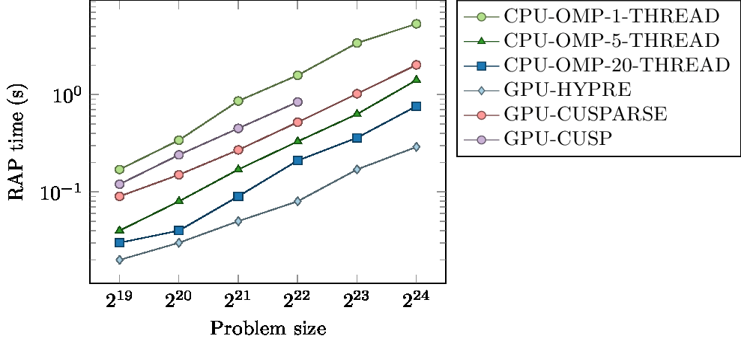
\includegraphics[width=3.9in]{projects/2.3.3-MathLibs/2.3.3.12-SUNDIALS-hypre/hypre-rap-1gpu.png}
	\caption{\label{fig:rap} Runtimes to generate a coarse grid operator for a 7pt 3d Laplace problem matrix on 1 V-100 GPU or Power 9 CPU with up to 20 OMP threads for various implementations}
\end{figure}

We also implemented a new integer datatype called HYPRE$\_$BigInt to avoid the requirement that all integers need to be converted to 64 bit integers when solving linear systems greater than 2 billions using the unstructured solvers. The new datatype allows to only convert variables that need to be 64 bit integers and improves memory usage and performance, as illustrated in Figure \ref{fig:mixed-int}.

\begin{figure}
\centering
	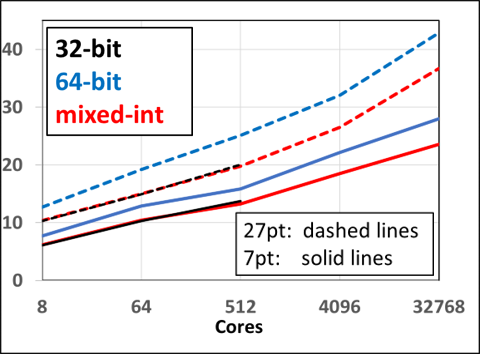
\includegraphics[width=2.5in]{projects/2.3.3-MathLibs/2.3.3.12-SUNDIALS-hypre/hypre-mixed-int.png}
	\caption{\label{fig:mixed-int} Weak scaling study on LLNL Linux cluster Quartz: Total runtimes in seconds for AMG-PCG using 1M points/core for 2 different 3D diffusion problems.The new mixed-int capability performs about 20-25 percent better than the 64 bit integer version while using less memory and is capable to solve larger problems than the 32 bit integer version.}
\end{figure}

\paragraph{Next Steps}

We will pursue the following tasks:

\begin{itemize}
\item We will continue to add new GPU capabilities to {\sl hypre}. This includes converting various components that are currently running only on the CPU to be usable on the GPU using CUDA or OpenMP 4.5. We will particularly focus on additional setup components, such as interpolation operators, to achieve better convergence.
\item We also plan on improving the efficiency of interfacing applications with {\sl hypre}'s solvers.
\end{itemize}
In addition, we will work with ECP application teams who are using {\sl hypre}, such as ExaWind, or would like to use it, to achieve best performance by tuning the solvers for them and potentially implementing suitable algorithmic changes. 


